\documentclass[twocolumn,10pt]{article}

% Standalone two-column source. Copy venue-specific class/style files from the
% licensed JCSA template beside this file if the venue requires its exact class.
\usepackage[margin=0.75in]{geometry}
\usepackage{amsmath}
\usepackage{booktabs}
\usepackage{graphicx}
\usepackage[hidelinks]{hyperref}
\usepackage[backend=biber,style=ieee]{biblatex}
\addbibresource{references.bib}
\graphicspath{{../results/runs/2026-08-23_tesla-t4_ca87722/artifacts/figures/}}

\title{CUDA Optimization of Fused Causal Softmax for Transformer Attention}
\author{Arwin Karir\\\small TODO(student): institution, program, and email}
\date{}

\begin{document}
\maketitle

\begin{abstract}
We study how CUDA work decomposition, reductions, warp communication, and
launch configuration affect fused FP32 causal scaled softmax and explicit
transformer attention. On one NVIDIA Tesla T4, all 88 structured softmax cases
passed. Across sequence lengths 128--2048, the final warp kernel was
3.22--8.92$\times$ faster than the row-serial kernel, 1.07--1.91$\times$ faster
than the shared-tree kernel, and 1.40--3.94$\times$ faster than equivalent
PyTorch eager softmax. Explicit custom attention improved by
1.54--2.31$\times$, but PyTorch scaled-dot-product attention remained faster at
all shapes. The results illustrate both the benefit of intra-row parallelism
and the end-to-end limit of optimizing one pipeline stage.
\end{abstract}

\section{Introduction}
Transformer attention~\cite{vaswani2017attention} applies softmax between two
matrix multiplications. Softmax requires row-wide maximum and sum reductions,
making it a compact case study in CUDA communication. This project evolves one
source file through Git history so that every design change is reviewable.

\section{Background}
For logits $x$, stable softmax computes
\begin{equation}
 p_i=\frac{\exp(x_i-m)}{\sum_j\exp(x_j-m)},\qquad m=\max_j x_j.
\end{equation}
Maximum subtraction avoids exponential overflow without changing the result.
CUDA warps exchange register values using shuffle operations, while shared
memory communicates across warps~\cite{nvidia2026cuda}. The target is narrower
than IO-aware full-attention fusion such as FlashAttention~\cite{dao2022flashattention}.

\section{Research Question}
How do GPU work decomposition, reductions, warp communication, and launch
configuration affect fused causal softmax, and how much do kernel gains
translate into complete transformer attention?

\section{Hypotheses}
We predicted that block-per-row work would outperform row-serial work at larger
shapes, warp reductions would outperform shared-memory trees, launch winners
would vary by shape, framework ordering could vary, and softmax speedup would
usually exceed attention speedup.

\section{Methodology}
The kernel fuses scaling, causal masking, stable exponentiation, reduction, and
normalization. Historical row-serial, shared-tree, and warp implementations are
recovered from Git commits. CUDA events measured 100 samples after 25 warmups.
Softmax used FP32, eight batch-head rows per sequence position; attention used
batch 1, eight heads, and head dimension 64. Sequence lengths were 128, 255,
512, 768, 1024, 1536, and 2048. Correctness used fixed tolerances of
$10^{-5}$ relative and $10^{-6}$ absolute.

\section{CUDA Implementation}
The first mapping assigns a row to one thread. The block mapping distributes
columns using thread-strided access and combines thread-local partials through
shared-memory trees. The final mapping uses warp shuffles, stores one value per
warp in a compact shared array, and lets the first warp finish each block-wide
reduction. The causal predicate and stable maximum subtraction stay in-kernel.

\section{Experimental Setup}
The measured clean commit is \texttt{ca87722a}. The environment was a Tesla T4
(compute capability 7.5), PyTorch 2.11.0+cu128, CUDA toolkit 12.8, and Python
3.13.15. All results are from one Google Colab session.

\section{Results}
All 88 structured softmax cases passed; maximum absolute error and maximum row
sum error were both $3.5763\times10^{-7}$. Figure~\ref{fig:historical} shows
3.22--8.92$\times$ speedup over row serial and 1.07--1.91$\times$ over the
shared tree. The custom kernel was 1.40--3.94$\times$ faster than PyTorch eager
and faster than steady-state \texttt{torch.compile} for six of seven shapes.
At length 2048, \texttt{torch.compile} was approximately 2.1\% faster.

\begin{figure}[t]
  \centering
  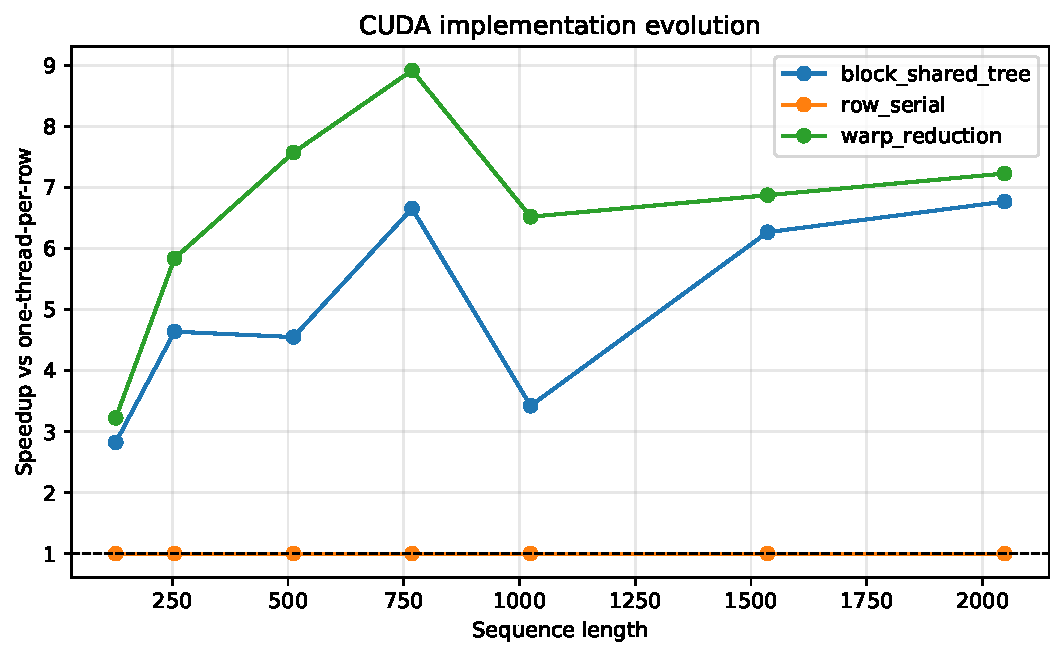
\includegraphics[width=\columnwidth]{fig_historical_speedup.pdf}
  \caption{Historical kernel speedup from matched raw CUDA-event samples.}
  \label{fig:historical}
\end{figure}

The 128-thread launch won five shapes, 256 threads won two long shapes, and 512
threads won none. The experiment's relative-latency rule selected 128 threads.

\section{Transformer Attention Experiment}
The custom path explicitly computes $QK^T$, custom softmax, then $PV$. It was
1.54--2.31$\times$ faster than explicit eager attention. Kernel speedup exceeded
attention speedup at six of seven lengths. PyTorch SDPA~\cite{pytorch2026sdpa}
was 1.25--2.53$\times$ faster than the explicit custom path at every shape.

\begin{figure}[t]
  \centering
  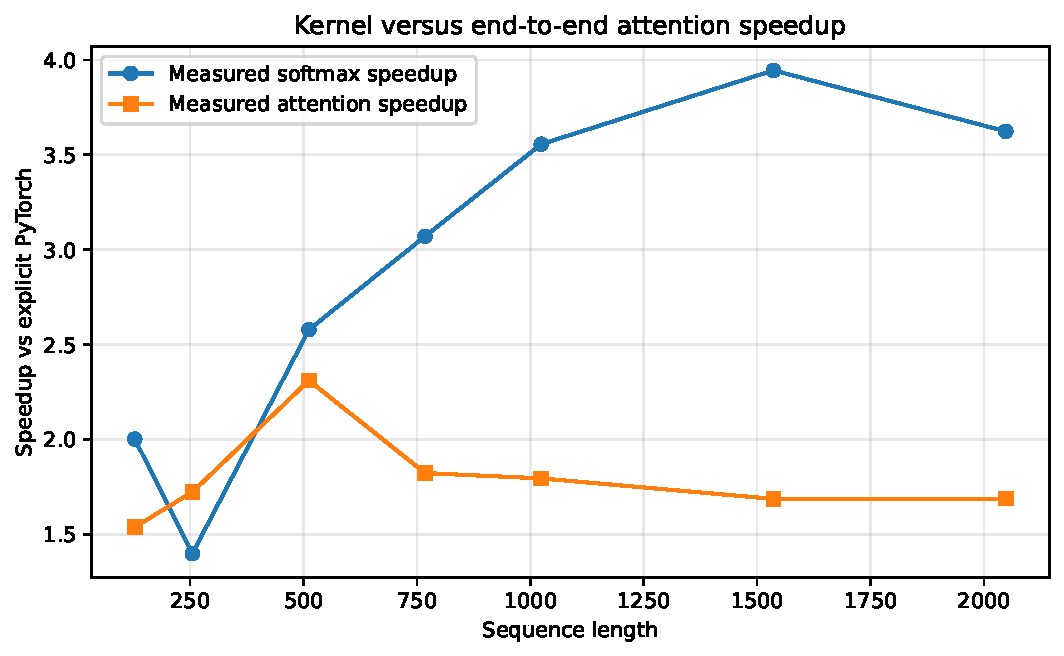
\includegraphics[width=\columnwidth]{fig_kernel_vs_attention_speedup.pdf}
  \caption{Softmax-only versus explicit-attention speedup.}
  \label{fig:translation}
\end{figure}

\section{Profiling Analysis}
\textbf{Measured:} At length 512, PyTorch Profiler~\cite{pytorch2026profiler}
reported 110.207 $\mu$s for the fused kernel. Nsight Compute
~\cite{nvidia2025nsight} reported 106.976--107.584 $\mu$s, 24 registers per
thread, 16 bytes dynamic shared memory, 48.33--48.79\% peak DRAM throughput,
and 56.72--57.00\% peak SM throughput across four profiled launches.

\textbf{Interpretation:} The compact shared footprint agrees with the intended
warp design, but these percentages alone do not establish a unique bottleneck.
Profiler captures are not substituted for steady-state benchmark medians.

\textbf{Next experiment:} Profile matched historical kernels and repeat on a
second architecture.

\section{Discussion}
Work decomposition produced the largest gain; warp communication then improved
the already parallel block design. Launch winners varied with shape. Attention
results follow the qualitative limit described by Amdahl's law
~\cite{amdahl1967validity}: unchanged matrix multiplications bound application
speedup. Measured and modeled attention values remain separate.

\section{Limitations}
This study covers FP32 forward causal softmax, one head dimension, one GPU, and
one session. It excludes backward execution, mixed precision, dropout,
arbitrary masks, replication across sessions, and cross-architecture results.
Historical builds required a documented header-only CUDA 12.8 compatibility
include. Percentiles describe samples from this run, not environment-level
confidence intervals.

\section{Future Work}
Repeat on newer architectures and independent sessions; add FP16/BF16 and
backward analysis; profile matched historical kernels; vary head dimensions;
and compare specialized library operators under equivalent work.

\section{Conclusion}
CUDA mapping and communication choices substantially improved the measured
softmax kernel and explicit attention, but a production fused SDPA baseline
remained faster. Kernel optimization is valuable but must be judged inside the
complete application path.

\section*{Artifact Availability}
Raw samples, environment metadata, figures, profiler exports, and the executed
notebook are preserved under
\texttt{results/runs/2026-08-23\_tesla-t4\_ca87722/}.

\printbibliography
\end{document}
